\documentclass{IEEEtran}
\usepackage[utf8]{inputenc}
\usepackage[alsoload=synchem,load=named]{siunitx}
\usepackage{graphicx}
\usepackage{amsmath}
\usepackage{booktabs, tabularx}
\usepackage{hyperref}
\usepackage{listings}
\usepackage{physics}
\usepackage[citestyle=ieee,sorting=none,bibencoding=utf8,backend=biber]{biblatex}

\graphicspath{{images/}}
\bibliography{bibliography}

\author{J.R. Powers-Luhn}
\title{Principal Component Analysis of Body Composition Measurements}
\date{October 2nd, 2018}

\DeclareSIUnit\year{yr}
\DeclareSIUnit\inch{in}

\begin{document}
\maketitle

\begin{abstract}

The generation of physical models suffers from the presence of noise in the measured quantities. Simple models such as linear regression assume that the input parameters are noiseless and further assume that they are linearly independent. Real-life data rarely satisfies the latter assumption and never satisfies the former. A technique for compensating for this, principal component analysis, is examined and applied to body composition measurements in an attempt to predict body fat percentage. The dataset is transformed into a principal component space of orthogonal components and these are used to generate regression models of the data. This method underperformed naive linear regressions with a root mean squared error of \num{4.72}\% but was comparable to a previously reported linear-in-parameters fit with an error on the same validation set of \num{4.79}\%.

\end{abstract}

\section{Introduction}

With the advent of automated data collection systems, datasets have become both deeper (with more granular data recorded at the second or sub-second level thanks to digital storage) and wider (with hundreds or thousands of sensors querying a system at once). These sensors are still subject to noise and may measure correlated quantities. Choosing which combination of sensors to include as inputs in a model scales in proportion to the number of sensors squared, making the creation of useful models grow rapidly more complex. This can be addressed by dimensionality reduction techniques such as principal component analysis (PCA). 

Principal component analysis is a linear transformation of a dataset. The measured input variables are used to generate an orthogonal spanning set of principal components that covers the input space. Since the transformation is linear it can be applied to future measurements in the dataset without updating the parameters. The columns of the transformation matrix are referred to as principal components; the products of the input measurements and the principal component transformation matrix are referred to as loading vectors or loadings. Principal component analysis has the additional design benefit of ordering each component based on the variance in the input data. This allows for dimensionality reduction with little loss of variance. Further, the rejection of low-variance components in the transformed space allows for more stability in the model by reducing the condition number of the matrix of input measurements, $\frac{\lambda_{max}}{\lambda_{min}}$.

As mentioned before, the principal components are calculated in order of the variance that they capture from the input data. Since the output data is not considered in the transformation, this is an unsupervised algorithm. In a similar fashion to the selection of inputs for a linear regression, principal components may show higher or lower correlation to an output variable, and this can be determined in the same ways (correlation matrix, scatter plots). Since the principal components are orthogonal by design, there is no need to determine the correlation between them--the calculation can be made for each column vector in the scores matrix against the output variable.

A final advantage of PCA is apparent if the assumption is made that the variance in the measured data exceeds the variance introduced by the noise in the measurements. This means that by rejecting loadings that correspond to low-variance principal components, the effect of noise on regression models can be reduced.

\section{Methodology} 

A dataset consisting of 247 samples with fifteen measurements recorded for each participant was obtained \cite{Penrose1985}. The first fourteen measurements were age, weight, adiposity index, and various circumference measurements. The last measurement was body fat percentage. Since many of the circumference measurements showed a high correlation (e.g. wrist and forearm circumference) principal component analysis was performed in order to isolate the varying components. The data set was split into training, testing, and validation sets by randomly sampling rows such that 70\% of the data was placed in the training set and 15\% each placed in the testing and validation set. The random number generator used to sample the rows was saved for reproducibility. 

Principal component analysis consists of a linear transformation from the measured units (in this case, a fourteen-dimensional space spanned by non-orthogonal measurements) into a new space where the unit vectors are orthogonal to each other. This process has the additional property that the spanning set that is so derived is ordered from highest to lowest variance from the original data. If the noise in a measurement can be assumed to be smaller in variance than the measured quantities, this means that the noise will be isolated to the later vectors.

In order to derive the new spanning set, the input data is transformed to have a mean of zero (and, optionally, a standard deviation of one) and the covariance matrix of the scaled input measurements is taken. If the mean centering step is omitted then the first principle component will be a vector from the origin to the mean in every dimension of the data. This is then decomposed into equation \ref{eq:eigenvalue_solution}\footnote{As shown by Dianat and Saber\cite{dianat2016}}:

\begin{align}
	\mathbf{C} \propto \mathbf{X}^T \mathbf{X} = \mathbf{W} \mathbf{\Lambda} \mathbf{W}^T
	\label{eq:eigenvalue_solution}
\end{align}

where \textbf{X} is the original sample (where each column represents a measurement and each row represents a sample), $\mathbf{\Lambda}$ represents a diagonal matrix of the eigenvalues, and $\mathbf{W}$ represents the matrix which transforms the rows from \textbf{X} into the new space. This is performed in such a fashion that the eigenvalue/eigenvector pair selected is the one that also captures the maximum amount of variance from the original data. This gives the first principal component vector. Subsequent loadings must also satisfy the condition that they be orthogonal to the loadings calculated before them. This is satisfied by first removing the already-calculated loadings from $\mathbf{X}$, then repeating the process on the new measured value (as in equations \ref{eq:later_pc1} and \ref{eq:later_pc2}). This can be repeated up to the minimum of the number of columns or the number of rows in $\mathbf{X}$. These vectors can be assembled into the matrix $\mathbf{W}$ which can transform measurement vectors from $\mathbf{X}$ into the loadings. The eigenvalues are also proportional to the amount of variance captured by the corresponding component. These eigenvalues can be normalized (equation \ref{eq:eigen_norm}) to determine the fraction of the total variance carried by each principal component.

\begin{align}
	\mathbf{X}_k &= \mathbf{X} - \sum_{i=0}^{k-1} \mathbf{X} \mathbf{w}_i \mathbf{w}_i^T \label{eq:later_pc1}\\
	\mathbf{w}_k &= \operatornamewithlimits{argmin}\limits_{||\mathbf{w}_k||} \frac{\mathbf{w}^T \mathbf{X}_k^T \mathbf{X}_k \mathbf{w}}{\mathbf{w}^T \mathbf{w}}
	\label{eq:later_pc2}
\end{align}

\begin{equation}
	\left| \lambda_i \right| = \frac{\lambda_i}{\sum_{j=1}^n \lambda_j}
	\label{eq:eigen_norm}
\end{equation}

Because the PCs are orthogonal to each other, it is possible to exclude individual columns from the transformed. This is equivalent to excluding the input from an individual sensor from a regression but with the added benefit that later loadings correspond to lower variance. If the assumption that the noise is lower variance than the measurements, this means that noise can be excluded simply by eliminating the low-variance vectors. In order to explore this, principal components were excluded based on three different parameters. First components which cumulatively captured at least 90\% of the variance (calculated as the first $n$ loadings such that $\operatornamewithlimits{argmin}\limits_{n} \sum_{i=0}^{n-1} \left| \lambda_i \right| \geq 0.9$. Second, components representing at least 1\% of the variance from the original sample ($\left| \lambda_i \right| \geq 0.01$) were isolated. Finally, principal components that were determined to be correlated with the output variable (body fat percentage) were isolated and used. The correlation between each PC and body fat percentage was calculated and the PCs were sorted in that order. Regressions models were generated by progressively adding the PCs in the order of their (absolute value of) correlation. The error of each of these models on the test set was plotted.

All models were compared to a regression of all PCs (equivalent to a regression of all of the original input variables).

\section{Results}

The input data were transformed into the PC space. The first four principal components were visually examined to see of what they consisted (see figure \ref{fig:first_four_pca}). All inputs were included in the first component except age--the variable least correlated with the other inputs. All other variables were included reduced by a factor of approximately \numrange{0.2}{0.3} except height, which was the second lest correlated. Age and height are more represented in PCA 1 and 2 (PCA's were numbered starting with 0). 

\begin{centering}
\begin{figure}
\centering
\begin{center}
	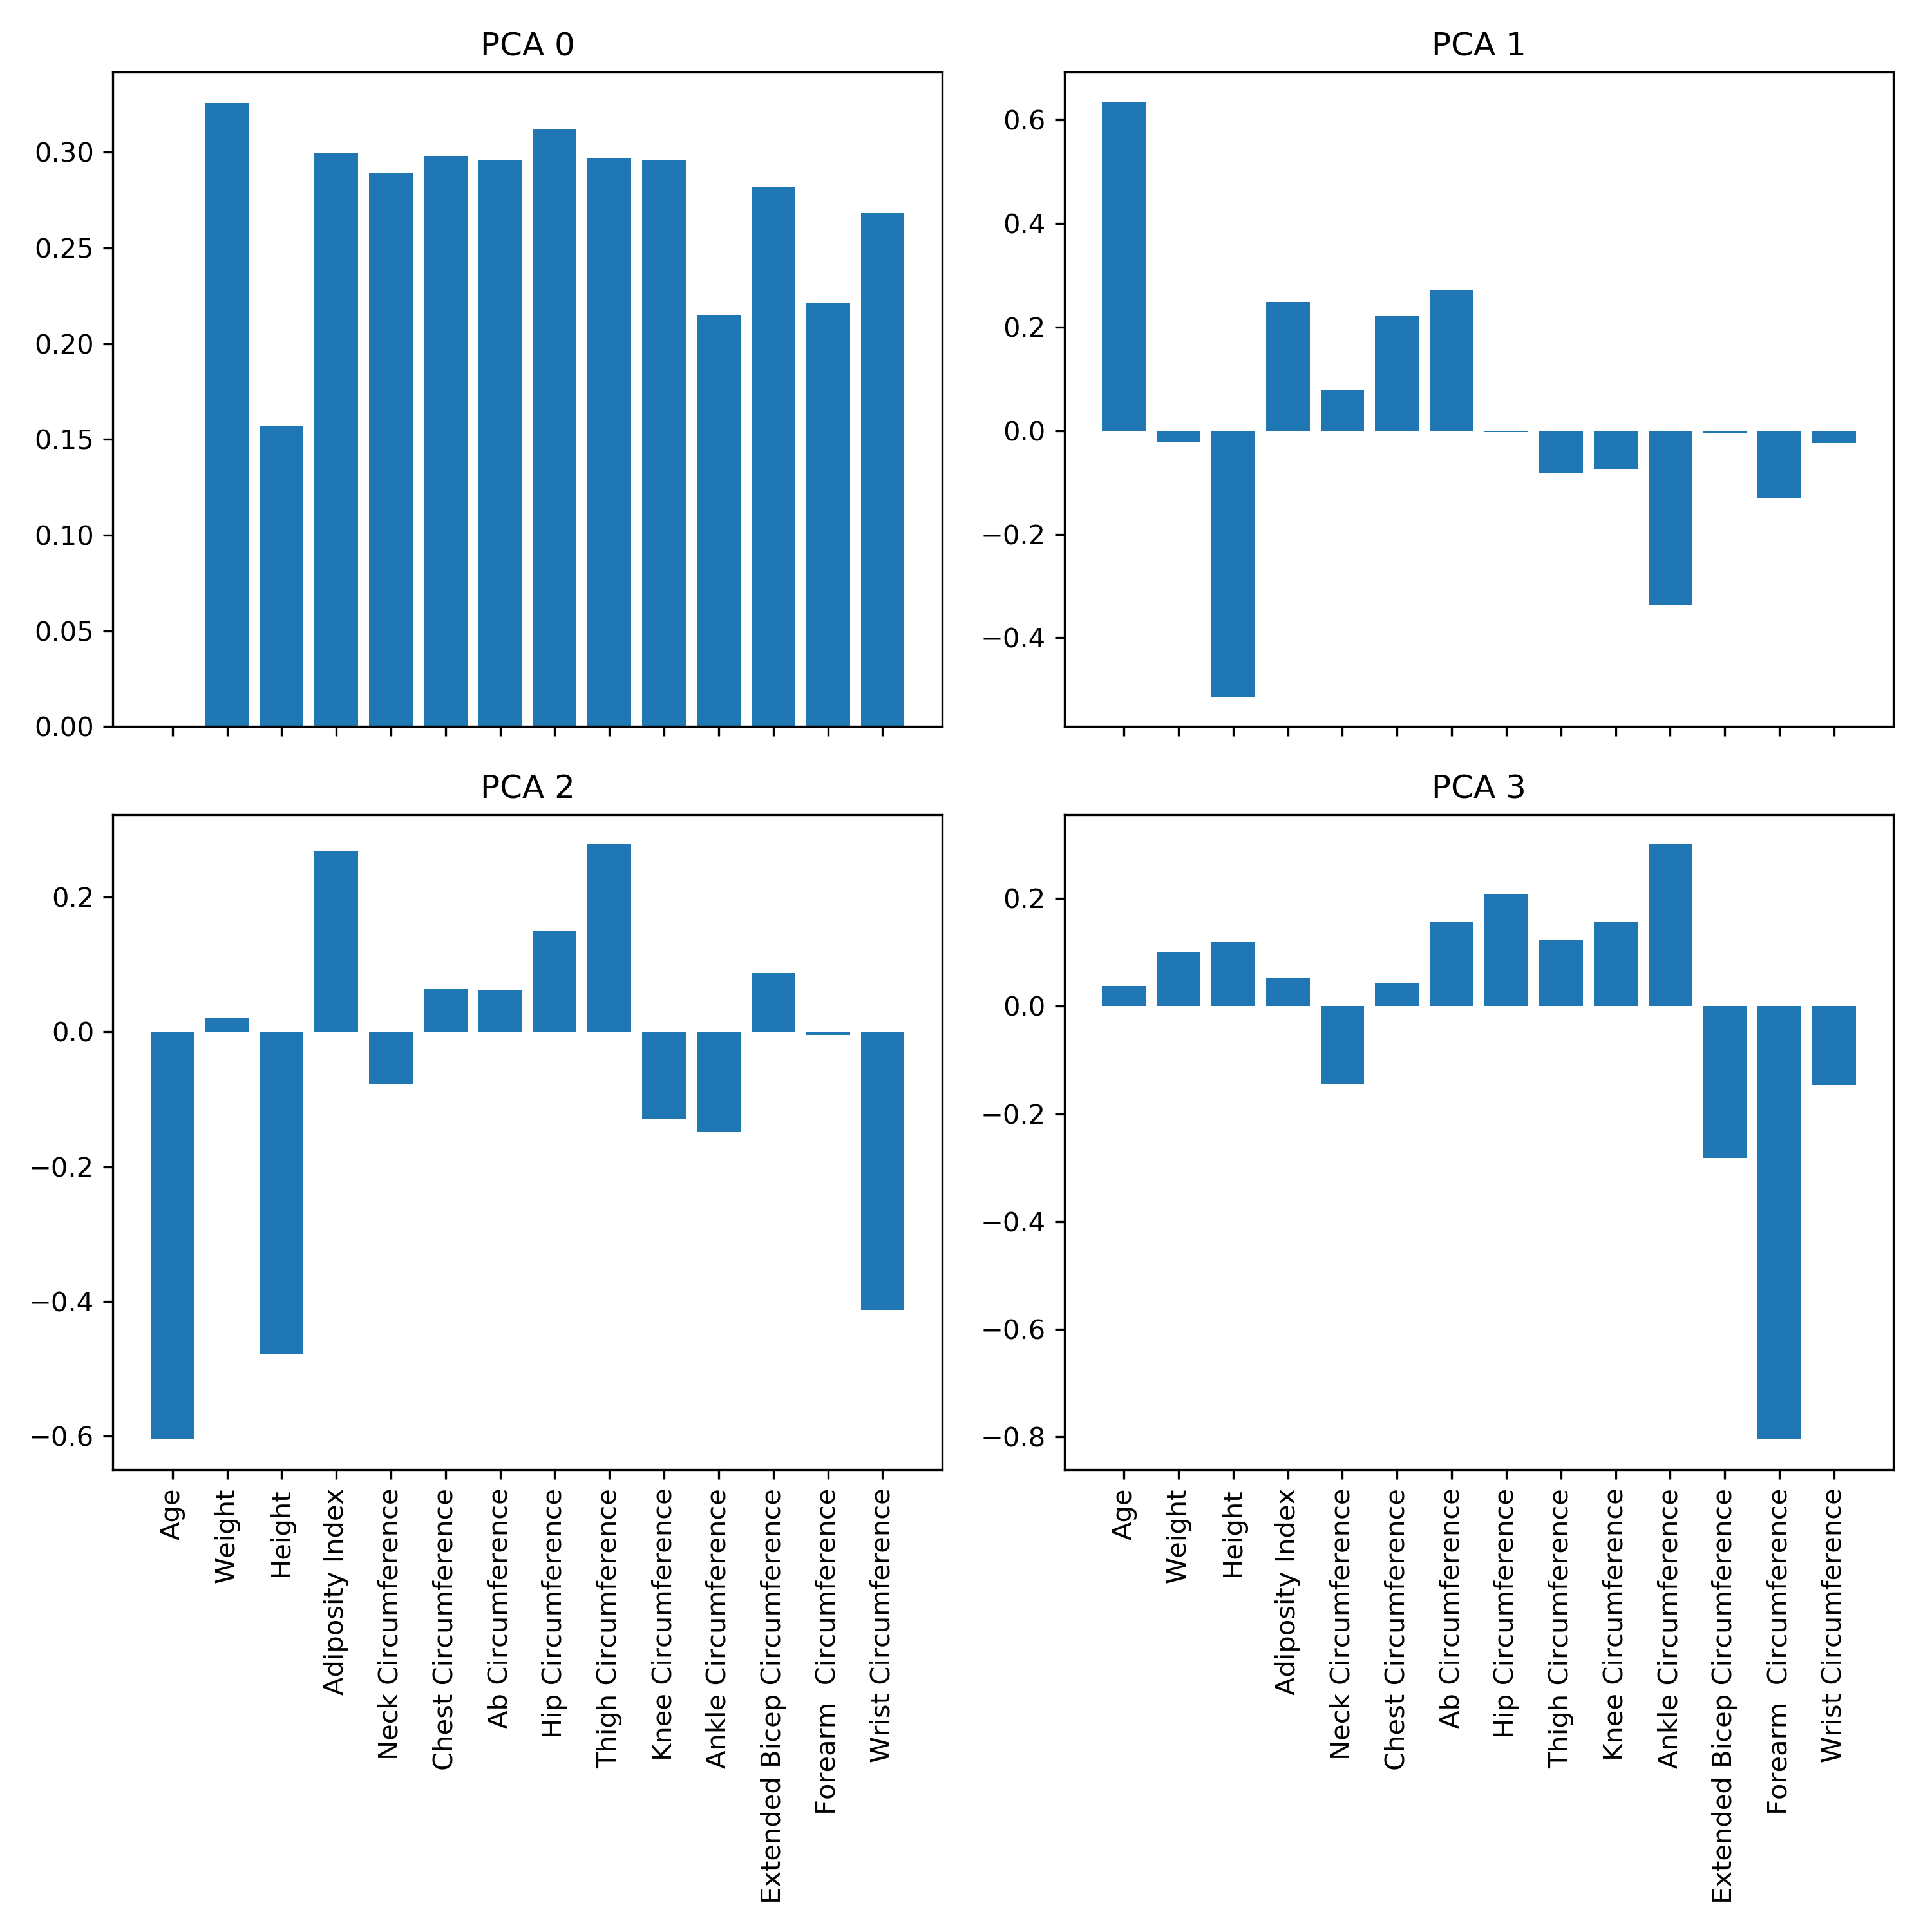
\includegraphics[width=0.5\textwidth]{first_four_pca}
	\caption{The first four principal components, capturing approximately 90\% of the variance. Age does not contribute to the first principal component, likely because it does not covary with the other measured values.\label{fig:first_four_pca}}
\end{center}
\end{figure}
\end{centering}

A regression was performed against the loadings corresponding to the first five PC's. This corresponded to the PC's that carried \textgreater90\% of the variance from the original sample, as shown in figure \ref{fig:cumulative_variance}. The performance of this model was the worst of all the models tested with a root mean squared error (RMSE) on the test set of \num{5.03}.

\begin{centering}
\begin{figure}
\centering
\begin{center}
	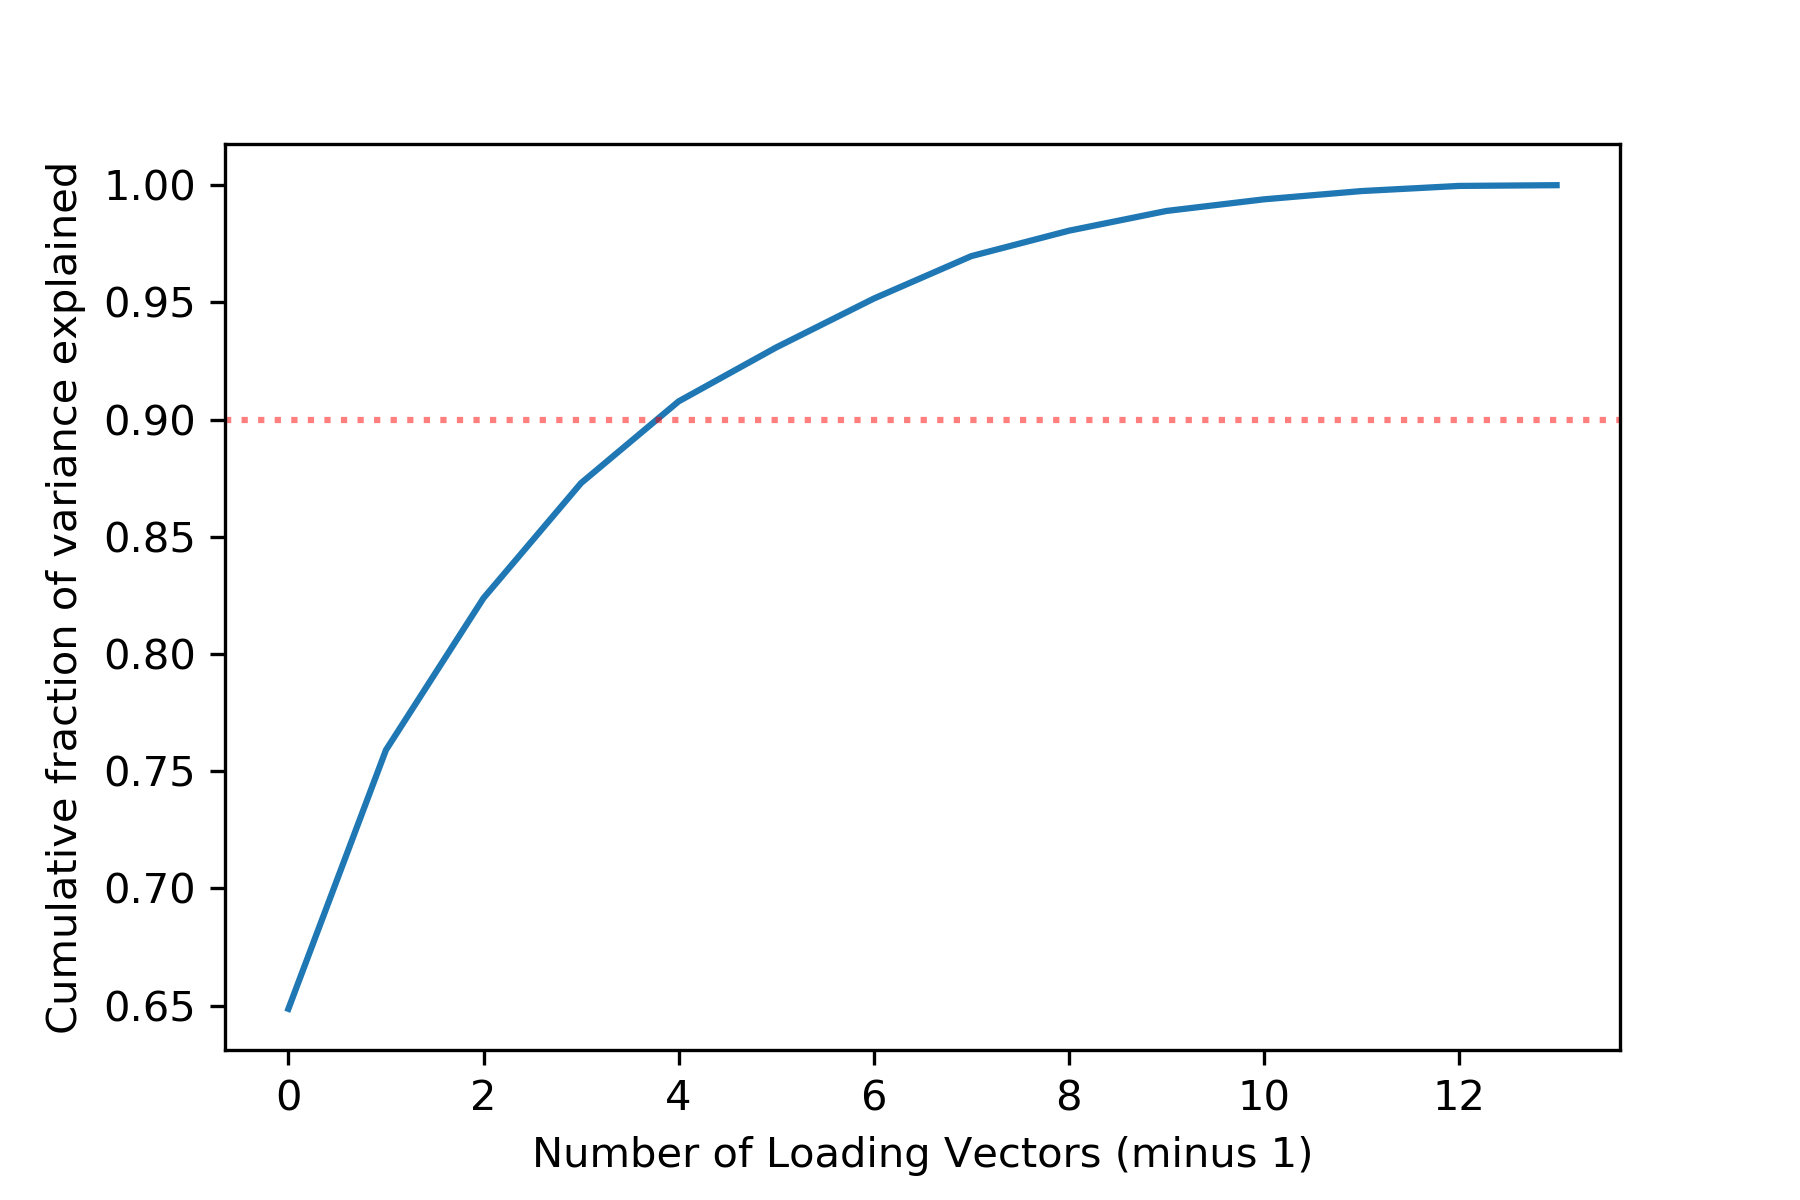
\includegraphics[width=0.5\textwidth]{cumulative_variance}
	\caption{Cumulative variance captured by the first $n$ principal components. Note that the plot starts at 0.65 and has a negative second derivative. This shows that subsequent principal components capture less and less of the variance.\label{fig:cumulative_variance}}
\end{center}
\end{figure}
\end{centering}

Next, a regression model was generated that used all principal components with eigenvalues corresponding to \textgreater1\% of the variance. This included PC's \numrange{0}{8} (figure \ref{fig:scaled_eigen}). This model performed better, with a RMSE of \num{4.50}. It seems that PC's \numrange{5}{8} contain information required to calculate body fat percentage so that including the loadings corresponding to these components improved the performance of the model. The condition number of this input was verified to be less than the rule of thumb value of 100 (figure \ref{fig:condition_number})

\begin{centering}
\begin{figure}
\centering
\begin{center}
	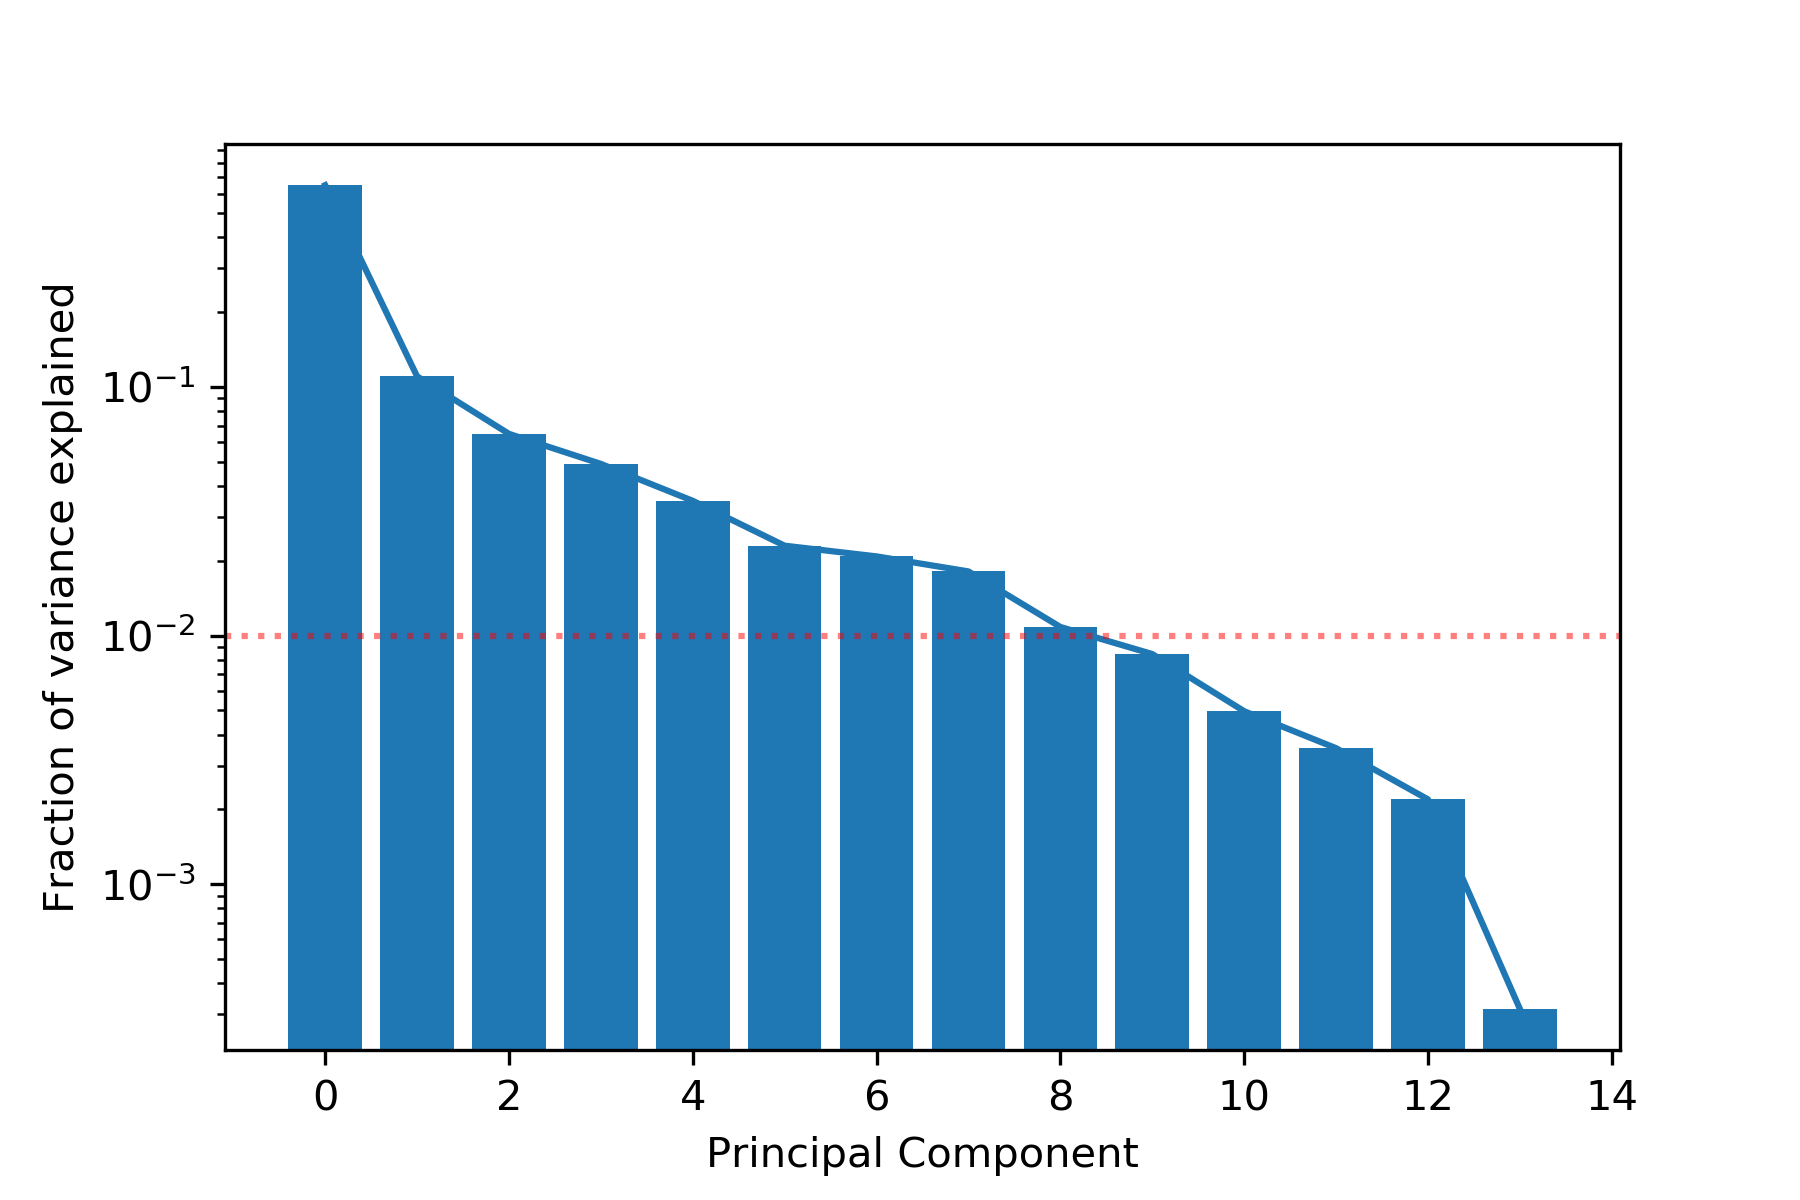
\includegraphics[width=0.5\textwidth]{fractional_variance_explained}
	\caption{Fraction of variance captured by each principal component. Each subsequent component captures less variance than its predecessor, necessitating a log scale. The red dotted line represents the 1\% variance threshold.\label{fig:scaled_eigen}}
\end{center}
\end{figure}
\end{centering}

Loadings that were correlated with the output variable were determined by calculating the absolute value of the correlation coefficient between each loading and body fat percentage (see figure \ref{fig:pca_correlation}). Linear regression against components with correlation values \textgreater0.3 showed degradation over the previous method attempted, with a test set RMSE of \num{4.92}. When the next most correlated loading column was included in the regression model performance improved, reaching a RMSE of \num{4.24}. Based on the improved test set performance, principal component scores were added to the model in the order in which they best correlated with the dataset. In each case consideration was given to the stability of the solution by examining the condition number of the input (see figure \ref{fig:condition_number_corr_ordered}) to verify that it did not significantly exceed the threshold value of 100. Test set error was minimized when components \numlist{0;1;5;11} were included in the model (see figure \ref{fig:selective_pcr_performance}). The condition number for this input matrix was calculated to be \num{184}--greater than the threshold value but by a factor of less than two. The risk of instability in the model was accepted based on the model's performance on the test set. An examination of plots of each loading column vs. body fat percentage showed no evidence of non-linear relationships so models incorporating these elements were not attempted.

\begin{centering}
\begin{figure}
\centering
\begin{center}
	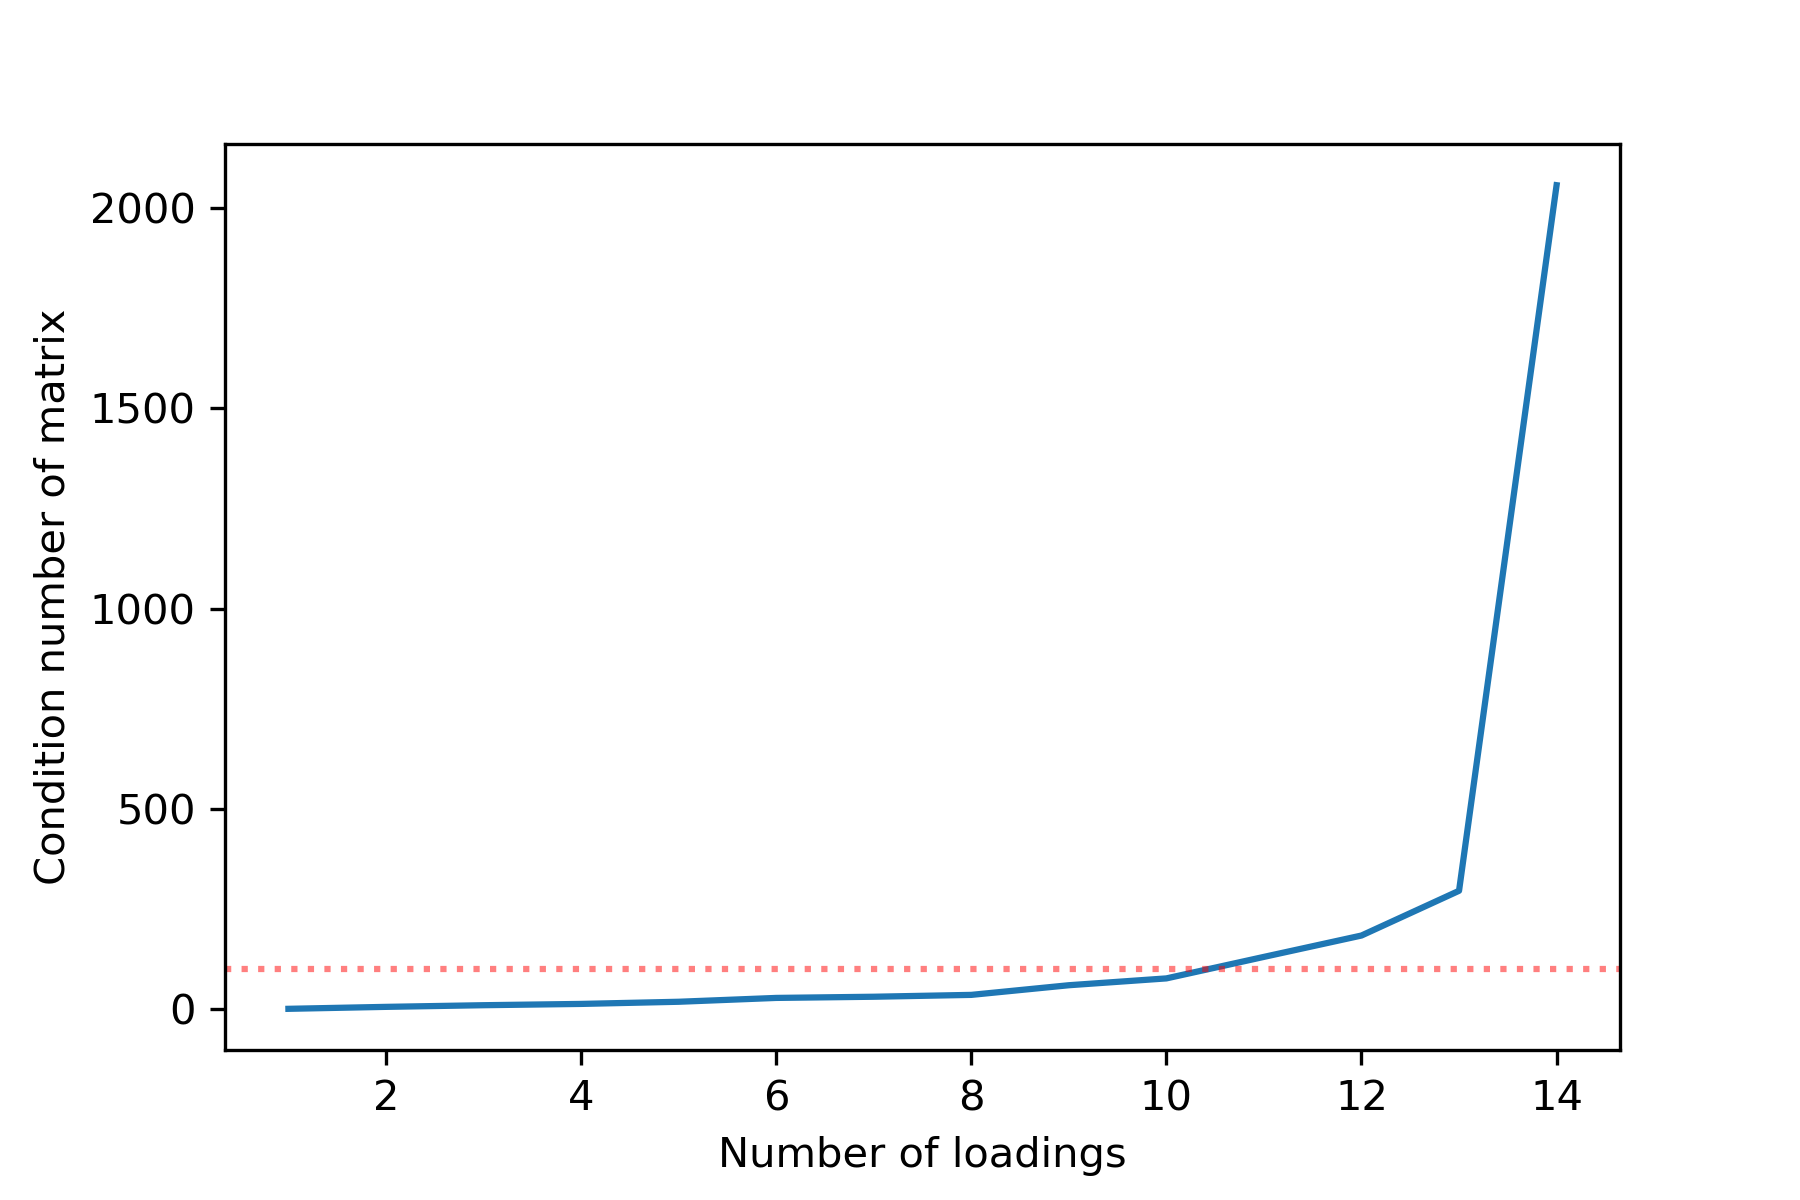
\includegraphics[width=0.5\textwidth]{condition_number}
	\caption{Condition number of the input matrix vs number of principal components included. The rule of thumb threshold value of 100 is denoted in red.\label{fig:condition_number}}
\end{center}
\end{figure}
\end{centering}

\begin{centering}
\begin{figure}
\centering
\begin{center}
	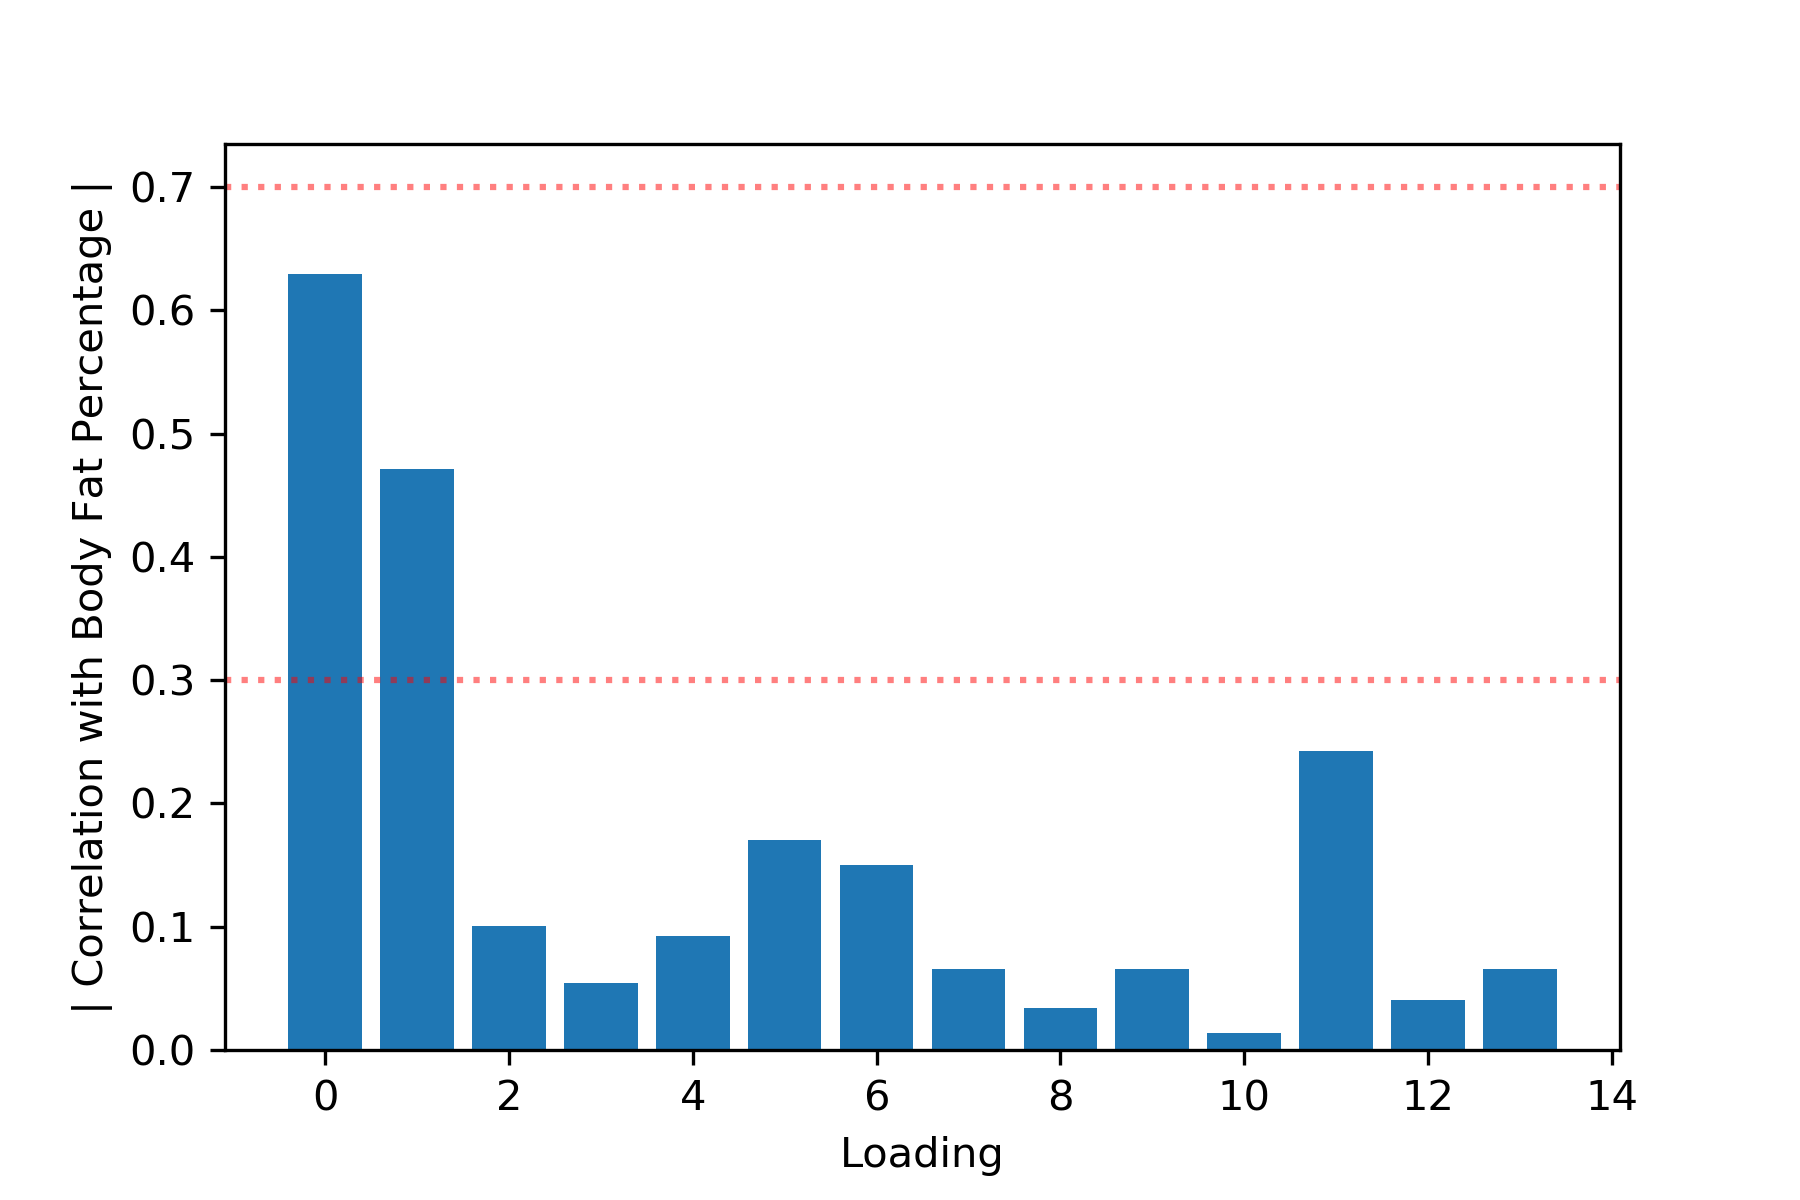
\includegraphics[width=0.5\textwidth]{pca_correlation}
	\caption{Correlation between each loading column and body fat percentage. No loading reached the threshold of "strongly correlated" (\textgreater0.7) and only the first two were correlated (\textgreater0.3).\label{fig:pca_correlation}}
\end{center}
\end{figure}
\end{centering}

\begin{centering}
\begin{figure}
\centering
\begin{center}
	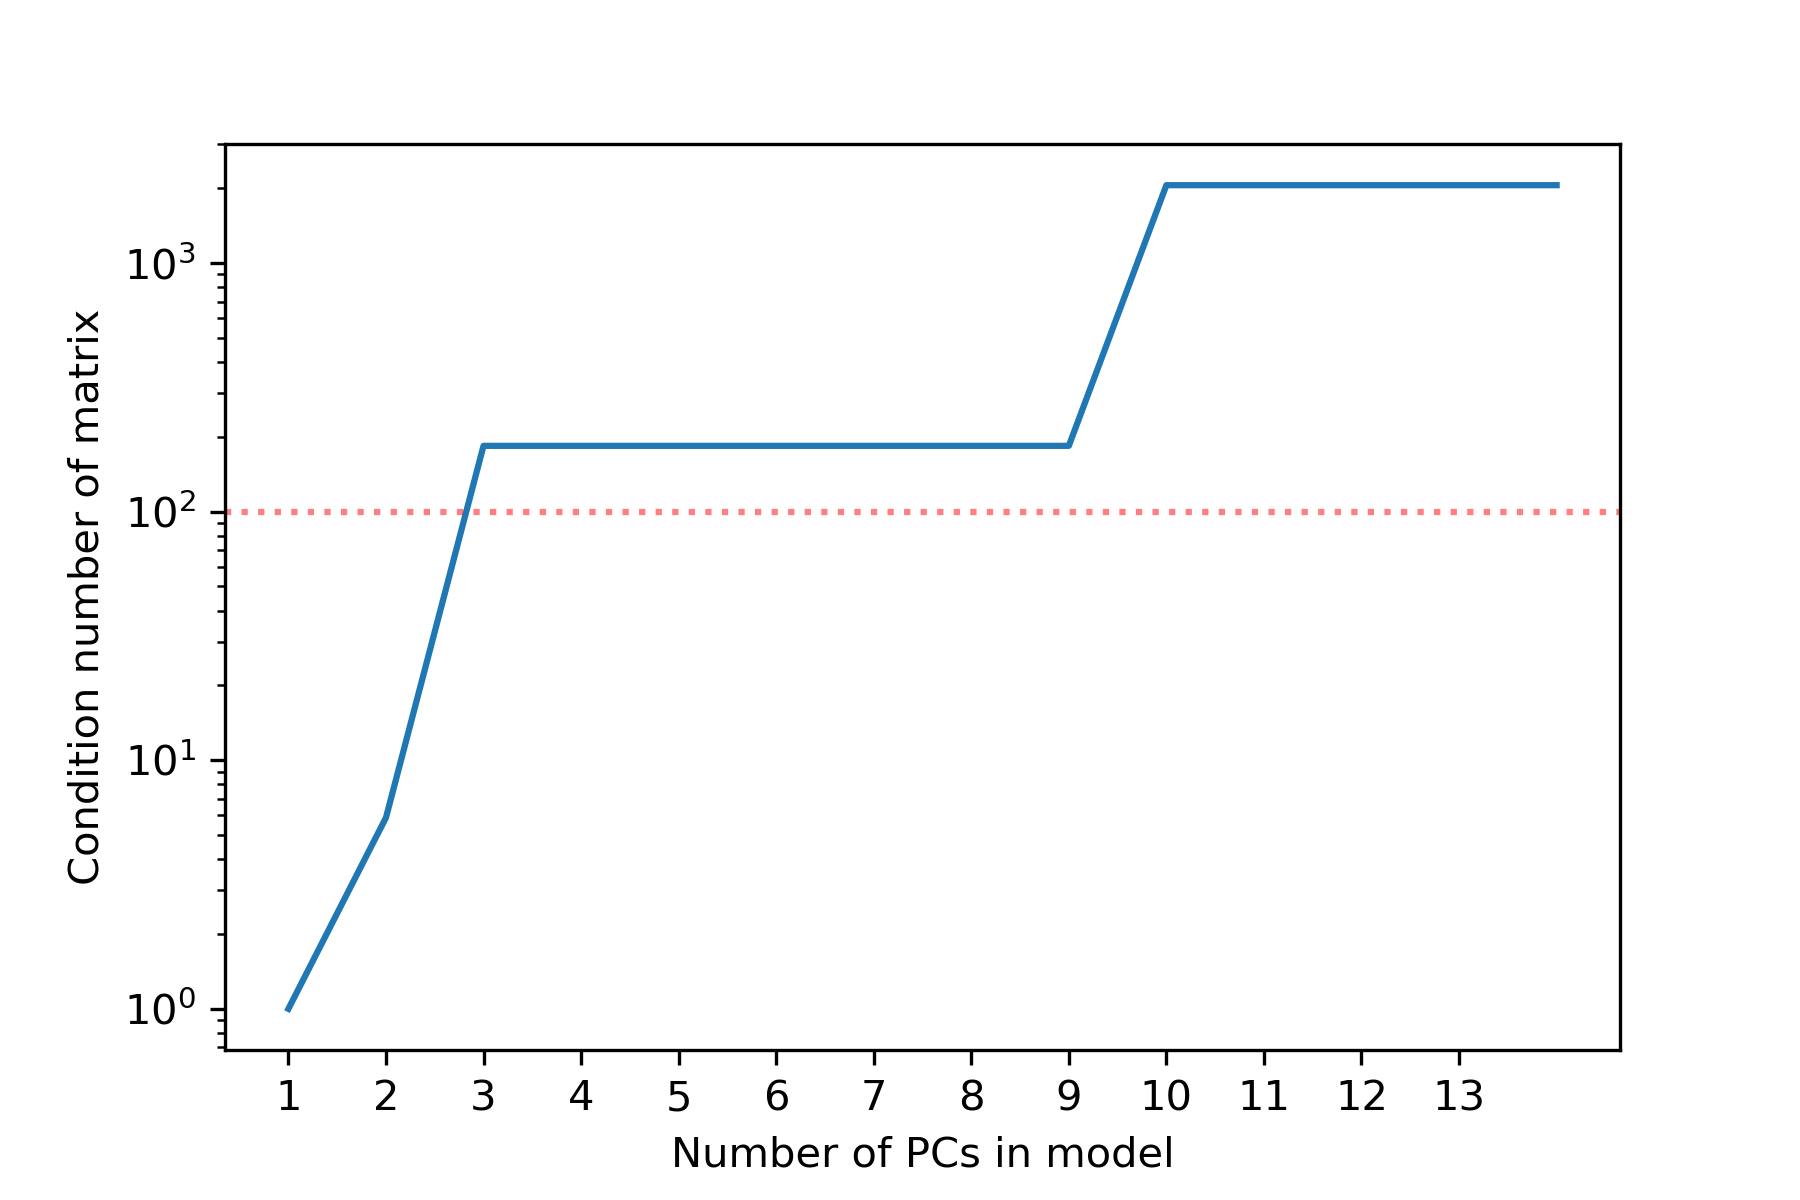
\includegraphics[width=0.5\textwidth]{condition_number_corr_ordered}
	\caption{Condition number of the input matrix vs number of principal components included when ordered by correlation. The rule of thumb threshold value of 100 is denoted by the dotted line.\label{fig:condition_number_corr_ordered}}
\end{center}
\end{figure}
\end{centering}

\begin{centering}
\begin{figure}
\centering
\begin{center}
	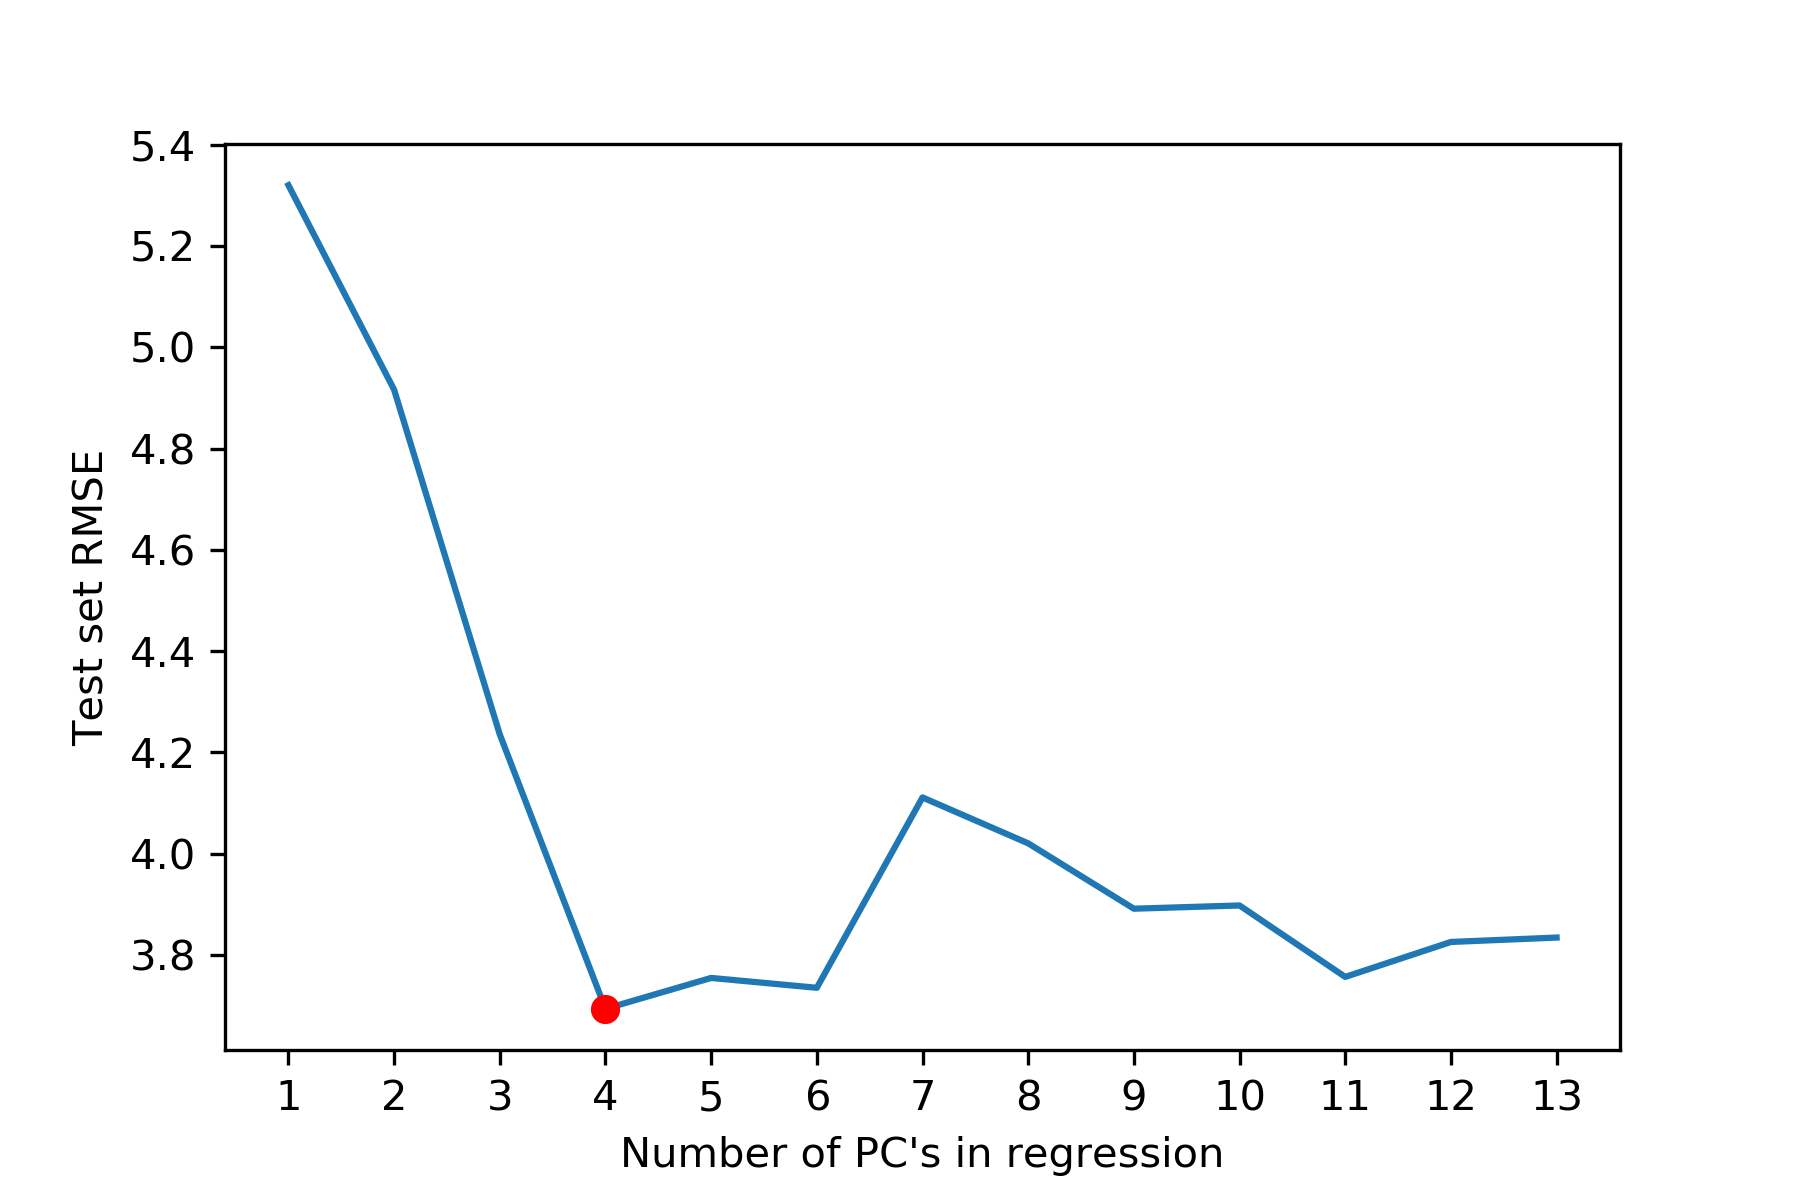
\includegraphics[width=0.5\textwidth]{selective_pcr_performance}
	\caption{Performance of linear models generated by including the $n$ best correlated principal components. A global minimum is found when four components are included, but local minima appear later as well.\label{fig:selective_pcr_performance}}
\end{center}
\end{figure}
\end{centering}

Finally, a principal component regression of all components was performed to test that performance. This was not expected to perform well, as it was mathematically equivalent to a linear regression using the original inputs. This model, however, outperformed all but one of the PCR models on the test set, with a RMSE of \num{3.83}.

Based on these results, a regression of the four most correlated loadings against body fat percentage was selected as the best model. Based on the visualization in figure \ref{fig:first_four_pca}, all measured values were present in the first two loading columns, implying that including additional columns introduces the potential to overfit the data. This was balanced against performance of the model on the test set. Figure \ref{fig:condition_number_corr_ordered} shows the condition number of the input matrix as additional components are included in the model. Since the components are not added in order of increased variance, the condition number of the matrix is no longer monotonically strictly increasing. Plateaus appear in regions following the addition of a correlated but low-variance principal component.

Test set performance for all models is summarized in table \ref{tab:results}.

The selected model had an error of \num{4.72} on the validation set. This was worse than the error on the validation set for a naive linear regression on all columns in the original data set (\num{4.19}) but slightly better than the validation error on a best-guess linear model (reported previously) of \num{4.79}.

\begin{centering}
\begin{table}
\caption{Results of Principle Component Regressions (test set)\label{tab:results}}
\begin{tabular}{lr}
\toprule
                                Model &      RMSE \\
\midrule
        PCR Capturing 90\% of Variance &  5.025354 \\
 PCR of loadings with \textgreater1\% of Variance &  4.500349 \\
    PCR of correlated loadings (\textgreater0.3) &  4.235354 \\
    PCR of correlated loadings (\textgreater0.2) &  4.916291 \\
       Best PCR sorted by correlation &  3.693315 \\
                  PCR of all loadings &  3.832659 \\
\bottomrule
\end{tabular}\end{table}
\end{centering}

\section{Conclusions}

While principal component analysis and principal component regression are promising tools for future analysis, they are not a panacea for all modeling problems. It is still helpful to have knowledge of the domain from which the data were taken in order to make intelligent decisions about which inputs to include. Still, the ability to isolate the high-variance elements of a dataset and perform regressions against this is a useful tool for data taken from real sensors. Principal component regression was able to perform as well on a validation set as a linear in parameters regression without the introduction of nonlinear components. At the very least this provides straightforward tool for the initial examination of a dataset to correct for covarying inputs and reduce noise.

%\nocite{*}
\printbibliography

\onecolumn
\section{Appendix}
Python code used to perform calculations and generate graphics.
\lstset{frame=single}
\lstinputlisting[language=python]{appendix/appendix.py}

\end{document}